\documentclass[11pt]{book}
\usepackage[utf8]{inputenc}
\usepackage[T1]{fontenc}	
\usepackage[italian]{babel}
\usepackage[bottom=2cm, top=3cm, left=3cm, right=2cm]{geometry}
\usepackage{graphicx}

\parindent=0pt \bigskipamount=20pt

\begin{document}

\chapter{Linguaggi e macchine astratte}

%% Slide 1

Nel corso della nostra trattazione cercheremo di dare risposta ad
alcune domande fondamentali:

\begin{itemize}
\item Quali istruzioni esegue un elaboratore?
\item Quali problemi pu\`o risolvere un elaboratore?
\item Esistono problemi che un elaboratore non pu\`o risolvere?
\item Che ruolo ha il linguaggio di programmazione?
\end{itemize}

%% Slide 2

Introduciamo alcune definizioni:

\begin{itemize}
\item \textbf{algoritmo}: \`e una sequenza \textbf{finita} di passi
  che risolve \textbf{in tempo finito} una \textit{classe} di
  problemi.

\item \textbf{Codifica}: \`e la scrittura di un algoritmo attraverso
  un insieme ordinato di \textbf{frasi} (\textbf{istruzioni}) di un
  \textbf{linguaggio di programmazione} che specificano le azioni da
  compiere.

\item \textbf{Programma}: \`e un testo scritto in accordo alla
  \textbf{sintassi} e alla \textbf{semantica} di un linguaggio di
  programmazione. 

  \textbf{Nota}: il programma spesso sar\`a un algoritmo, ma pu\`o
  anche non esserlo e ci\`o accade quando un programma non termina,
  cio\`e quando prevede una sequenza di passi infinita. Un esempio \`e
  dato dai sistemi operativi che restano in esecuzione fino a quando
  non \`e l'utente a stopparli. In generale possiamo dire che non sono
  algoritmi i programmi che devono \textit{agire}, pi\`u che
  \textit{calcolare un risultato}.

\end{itemize}

%% Slide 3 e 4

Escludiamo per ora l'eccezione appena presentata e consideriamo quindi
un programma come la formulazione testuale di un algoritmo che risolve
un dato problema (o meglio una data classe di problemi). Partendo dai
dati in ingresso, svolgendo in sequenza tutte le azioni previste
dall'algoritmo, si ottiene il risultato dell'elaborazione. Ci\`o
presuppone l'esistenza di un'entit\`a che effettivamente esegua i
passi, quindi di un \textbf{automa esecutore}. Definiamo l'automa
esecutore come una macchina astratta capace di eseguire le azioni
specificate dall'algoritmo. L'automa esecutore riceve in ingresso
oltre ai dati anche l'algoritmo che dovr\`a essere espresso in qualche
linguaggio. L'automa dovr\`a perci\`o essere in grado di interpretare
il linguaggio. 

\vspace{20pt}
\begin{center}
\begin{tabular}{rcl}
& $\downarrow$ Algoritmo & \\
\cline{2-2}
Dati $\rightarrow$ & \vline ESECUTORE \vline & $\rightarrow$ Risultati \\
\cline{2-2}
\end{tabular}
\end{center}
\vspace{20pt}

Affinch\'e possa essere realizzabile l'automa deve soddisfare i
seguenti vincoli:

\begin{itemize}
\item se l'automa dev'essere composto da un \textbf{numero finito di
    parti};
\item ingresso e uscita devono essere denotabili attraverso un
  \textbf{insieme dinito di simboli}.
\end{itemize}

%% Slide 5

Non abbiamo ancora detto nulla sull'automa in s\`e, su come dev'essere
progettato, su come debba \textbf{computare}. Esistono vari approcci,
vari \textbf{sistemi formali} che definiscono in modo diverso la
\textbf{computabilit\`a}. Riepiloghiamo di seguito i principali
sistemi formali:

\begin{itemize}
\item \textbf{gerarchia di macchine astratte}: dall'automa a stati
  finiti alla macchina di Turing ed \`e il modello di computazione su
  cui ci concentreremo noi;
\item \textbf{approccio funzionale}: basato sul concetto di funzione
  matematica;
\item \textbf{sistemi di riscrittura}: che descrivono l'automa come un
  insieme di regole di riscrittura (o inferenza) che trasformano frasi
  in altre frasi.
\end{itemize}

%% Slide 6

\section{La gerarchia di macchine}

La gerarchia di macchien \`e cos\`i composta (indicando le macchine
dalla meno potente alla pi\`u potente:

\begin{enumerate}
\item reti combinatorie;
\item automi a stati finiti;
\item macchina a stack;
\item macchine di Turing.
\end{enumerate}

Diversi macchine hanno diverse capacit\`a risolutive. Se neanche la
pi\`u potente riesce a risolvere un problema, allora potrebbe non
essere risolubile.

% Slide 7

\subsection{La macchina base, combinatoria}

Si trata di una rete definita formalmente dalla tripla: \texttt{I, O,
  mfn} dove gli elementi che la compongono sono:

\begin{itemize}
\item \texttt{I}: insieme \textbf{finito} dei simboli di ingresso;
\item \texttt{O}: insieme \textbf{finito} dei simboli di uscita;
\item \texttt{mfn: I -> O}: funzione macchina
\end{itemize}

Esempi di queste reti sono le \textbf{porte logiche}. Se prendessimo
come esempio una porta logica a due ingressi, avremmo
$I=\{\{0,1\} \times \{0, 1\}\}$ e $O=\{0,1\}$.

% Slide 8

La macchina combinatoria \`e una rete semplicissima e in quanto tale
presenta dei limiti:

\begin{itemize}
\item risolvere problemi con tale macchina comporta
  l'\textbf{enumerazione completa} di tutte le possibili
  configurazioni di ingresso ed indicare il corrispondente valore di
  uscita;
\item si tratta di un dispositivo puramente combinatorio, quindi
  \textbf{inadatto per problemi che richiedano memoria interna}.
\end{itemize}

% Slide 9

\subsection{L'automa a stati finiti}

Abbiamo detto che uno dei limiti delle macchine base \`e
l'impossibilit\`a di risolvere problemi che richiedano memoria. Con
gli automi a stati finiti si introduce proprio il concetto di memoria
grazie ad un numero finito di \textbf{stati interni}.

L'automa a stati finiti \`e definito dalla quintupla: \texttt{I, O, S,
  mfn, sfn}. Questi simboli indicano:

\begin{itemize}
\item \texttt{I}: come per le macchine base \`e l'insieme finito dei
  simboli di ingresso;
\item \texttt{O}: come per le macchine base \`e l'insieme dinito dei
  simboli di uscita;
\item \texttt{S}: \`e l'insieme finito degli \textbf{stati};
\item \texttt{mfn}: $I \times S \rightarrow O$ \`e la funzione di
  macchina;
\item \texttt{sfn}: $I \times S \rightarrow S$ \`e la \textbf{funzione
    di stato futuro}.
\end{itemize}

%% Slide 10

L'uscita dipende ora dallo stato, pertanto si evince la capacit\`a
della macchina di tenere in memoria informazioni che, al pari dei dati
in ingresso, influenzano il risultato della computazione.

Anche l'automa a stati finiti, ovviamente, ha un limite: ha
\textbf{memoria finita}, quindi \`e inadatto a risolvere problemi che
non consentono di limitare a priori le sequenze di ingresso da
memorizzare. Un problema che possono risolvere le macchine a stati
finiti \`e quello del bilanciamento delle parentesi, tuttavia possono
farlo soltanto se il numero di parentesi non eccede il massimo numero
previsto in fase di progettazione dell'automa. Si dovrebbe quindi
conoscere a priori il massimo numero di parentesi che si possono
verificare per poter progettare l'automa senza rischiare
malfunzionamenti dovuti a input eccessivamente lunghi.

%% Slide 11

\subsection{La macchina di Turing}

Saltiamo per il momento le macchine a stack e concentriamoci sul
livello immediatamente seguente nella gerarchia: le macchine di
Turing, l'automa pi\`u potente a disposizione.

La macchina di Turing introduce un supporto di memorizzazione esterna,
un nastro illimitatamente espandibile, ed \`e definita dalla
quintupla: \texttt{A, S, mfn, sfn, dfn}. Questa volta gli alfabeti di
ingresso e di uscita (sempre finiti) sono considerati coincidenti ed
indicati con \texttt{A}. \texttt{mfn} ed \texttt{sfn} sono le funzioni
che abbiamo gi\`a visto prima (uscita e stato futuro), mentre la
\texttt{dfn} \`e la funzione di indirizzamento sul nastro: $A \times S
\rightarrow D = \{ Left, Right, None \}$.

%% Slide 12

%% Slide 13 

Risolvere un problema con la \textit{MdT} richiede quindi di:

\begin{enumerate}
\item definire un'opportuna rappresentazione dei dati iniziali sul
  nastro;
\item definire la parte di controllo (cio\`e le tre funzioni.
\end{enumerate}

Un esempio di problema risolvibile tramite le macchine di Turing \`e
il riconoscimento dei palindromi.

Secondo \textbf{Church-Turing} non esiste una macchina capace di
risolvere una classe di problemi pi\'u ampia rispetto alla macchina di
Turing, pertanto se un problema non \`e risolvibile con essa
probabilmente non pu\`o essere risolto in altro modo.

Se l'algoritmo non \`e cablato all'interno della MdT, ma va recuperato
dal nastro, allora si ha una macchina \textbf{general purpose}, anche
detta \textbf{Macchina di Turing Universale} (UTM). Si tratterebbe
quindi di una macchina programmabile. L'UTM sarebbe un interprete di
linguaggio in quanto interpreterebbe il programma presentato sul
nastro (che \`e espresso in un dato linguaggio). La UTM rivestirebbe
quindi il ruolo dell'automa esecutore presentato prima, svolgendo
soltanto le operazioni di \texttt{fetch}, \texttt{decode} ed
\texttt{execute}.

%% Slide 14 16-fine

\subsubsection*{UTM e macchina di Von Neumann}

Volendo fare un paragone fra l'UTM e la macchina di Von Neumann,
potremmo individuare le seguenti corrispondenze:

\begin{itemize}
\item leggere/scrivere un simbolo dal/sul nastro corrisponde a
  leggere/scrivere dalla/sulla memoria;
\item transitare in un nuovo stato interno corrisponde ad una nuova
  configurazione dei registri della CPU;
\item spostarsi sul nastro corrisponde a scegliere una cella di
  memoria su cui operare.
\end{itemize}

Dunque effettivamente si potrebbe dire che c'\`e una forte
corrispondenza fra le due macchine, tuttavia l'interazione con il
mondo esterno nella UTM manca completamente. L'UTM opera soltanto da e
verso il nastro. La Universal Turing Machine \`e quindi una
\textbf{macchina di pura computazione}.

\textbf{Computazione} e \textbf{interazione} sono dimensioni
ortogonali che vengono modellate separatamente ed espresse
(potenzialmente) da linguaggi distinti, il primo dei quali \`e detto
\textbf{linguaggio di computazione}, il secondo di
\textbf{coordinazione}. Mentre il linguaggio di computazione definisce
le primitive per elaborare le informazioni, il linguaggio di
coordinazione contiene le primitive di input/output di informazioni da
e verso il mondo esterno. All'interno di questo linguaggio troviamo il
\textbf{linguaggio di comunicazione} che definisce quali informazioni
vadano trasmesse.

\begin{figure}[h]
  \centering
  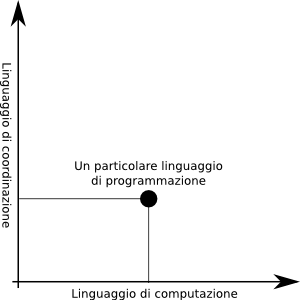
\includegraphics[width=.35\textwidth]{images/computazioneinterazione.png}
  \caption{Computazione e interazione}
  \label{computazioneinterazione}
\end{figure}

%% Slide 15

\subsection{Il Push Down Automaton}

\`E un automa pi\`u limitato rispetto alla MdT (e infatti la precede
nella gerarchia) e la differenza consiste nella presenza di una
memoria pi\`u limitata.

\end{document}